\documentclass[fleqn]{jbook}
\usepackage{physpub}
\usepackage{graphicx}
\begin{document}

\begin{question}{専攻 問題8}{石井}
\begin{subquestions}

\SubQuestion
1,1,1-トリクロロエタン分子(CH$_{3}$-CCl$_{3}$)のC-C単結合の周りの内部回転を考える。CCl$_{3}$基の慣性モーメントは大きいので止まっていると仮定して、CH$_{3}$基の回転運動を取り扱う。
\begin{subsubquestions}
\SubSubQuestion
CH$_{3}$基のC-C軸周りの慣性モーメントを求めよ。ただし、C-Hの核間距離を$r$、C-H結合とC-C結合のなす角度を$\theta$、水素原子の質量を$m$とする。

\SubSubQuestion
CH$_{3}$基がC-C軸周りに自由に回転しているとする。回転角を$\phi$として、回転運動のハミルトニアンを導け。また、それをもとにシュレディンガー方程式を解いて、エネルギー準位を求めよ。ただし、CH$_{3}$基のC-C軸周りの慣性モーメントは$I$としてよい。

\SubSubQuestion
実際はC-C軸周りの回転は自由回転ではなく、水素と塩素との立体反発のために相互が接近する位置でのポテンシャルエネルギーは高くなり、遠ざかる位置でのポテンシャルエネルギーは低くなる。それを
\[   V = \frac{V_{3}}{2}(1- \cos 3 \phi )  \]
で表す。ここで、$\phi$はポテンシャルの一つの極小を0にとっており、$V_{3}$はポテンシャルの極大と極小の差を表すパラメーターである。もし、$V_{3}$が十分大きければ、CH$_{3}$基のC-C軸周りの運動は、$\phi=0$の近傍で調和振動子になることを示し、そのエネルギー準位を求めよ。
\end{subsubquestions}

\SubQuestion
次に、1,2-ジクロロエタン分子(CH$_{2}$Cl-CH$_{2}$Cl)を考える。この分子の場合、C-C結合周りの回転異性体として、トランス型とゴーシュ型が存在する。これらは室温で相互に移り変わることができるので単離精製はできない。従って、室温の気体、液体は異なる構造を持つ2種類の回転異性体の混合物として理解できる。
\begin{subsubquestions}
\SubSubQuestion
トランス型とゴーシュ型の立体構造を図示せよ。できれば、Newman投影図を用いて表せ。

\SubSubQuestion
気体の1,2-ジクロロエタンの赤外線吸収スペクトルを測定したところ、C-Cl伸縮振動による吸収が、トランス型では$709~\text{cm}^{-1}$の1本、ゴーシュ型では$675~\text{cm}^{-1}$と$653~\text{cm}^{-1}$の2本が測定された。なぜ、ゴーシュ型ではC-Cl伸縮による吸収が2本見えるのに、トランス型ではC-Cl伸縮による吸収が1本しか見えないのかを、トランス型、ゴーシュ型の分子構造及び赤外線吸収のメカニズムをもとに説明せよ。

\SubSubQuestion
トランス型とゴーシュ型のエネルギー差$\Delta E$を求めたい。そのために様々な温度$T$で赤外線吸収スペクトルを測定し、トランス型のバンドの強度$I_{t}(T)$とゴーシュ型のバンドの強度$I_{g}(T)$を求めた。このデータから$\Delta E$を求める方法を説明せよ。

\SubSubQuestion
前問の実験の結果、気体状態ではトランス型が安定で、$\Delta E/hc$は$420~\text{cm}^{-1}$であることがわかった。C-C結合の回転角を$\phi$として、内部回転のポテンシャルエネルギー曲線を$\phi$の関数としてグラフに示せ。その際、ポテンシャルエネルギー曲線の極大値を決定する要因についても考慮せよ。また、トランス型、ゴーシュ型がどの$\phi$に対応するかを書き入れよ。

\SubSubQuestion
前問で示した$\Delta E$の時、290~Kにおける気体状態でのトランス型、ゴーシュ型の存在比率を求めよ。ただし、光速$c=3 \times 10^{8}$ m/s、プランク定数$h=6.6 \times 10 ^{-34}$ J$\cdot$s、ボルツマン定数$k=1.4 \times 10 ^{-23}$ J/K、自然対数の底$e=2.7$とする。
\end{subsubquestions}
\end{subquestions}

\end{question}
\begin{answer}{専攻 問題8}{石井}

\begin{subanswers}
\SubAnswer 
\begin{subsubanswers}
\SubSubAnswer
\parbox[t]{.5\linewidth}{
右の図より
\begin{align*}
I &= 3 \times m \times (r \sin \theta )^{2}  \\
  &= 3mr^{2} \sin ^{2} \theta 
\end{align*}
}
\parbox[t]{.5\linewidth}{
\begin{center}
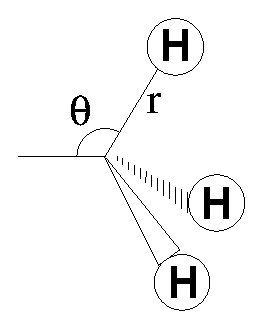
\includegraphics[height=3cm]{1999phy8-1.eps}\\
CH$_3$基
\end{center}
}


\SubSubAnswer
CH$_3$基において座標を以下のように定める。\\

\begin{minipage}{.45\linewidth}
\begin{center}
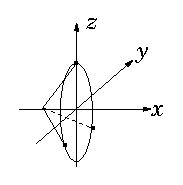
\includegraphics[width=3cm]{1999phy8-2.eps}
\end{center}
\end{minipage}
\begin{minipage}{.45\linewidth}
\begin{center}
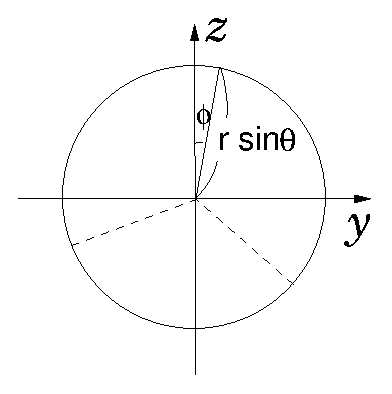
\includegraphics[width=3cm]{1999phy8-3.eps}
\end{center}
\end{minipage}\\

この系の古典的なラグランジアンは、
\[
L = \frac{1}{2}I\dot{\phi}^2
\]
である。また、
\[
p_\phi = \frac{\del L}{\del \dot{\phi}} = I\dot{\phi}
\]
となる。これを用いると、古典的なハミルトニアンは、
\[
H = p_\phi \dot{\phi} -L = \frac{1}{2I}p_\phi^2
\]
となる。従って、$p_\phi$を演算子で置き換えて、量子論的なハミルトニアンは、
\[
\hat{H} = \frac{1}{2I}\left(\frac{\hbar}{i}\frac{\del}{\del \phi}\right)^2
= -\frac{\hbar^2}{2I}\frac{\del^2}{\del \phi^2}
\]
となる。

これをもとにシュレディンガー方程式をたてると
\[
-\frac{\hbar ^{2}}{2I}\frac{\del ^{2} \Psi (\phi)}{\del \phi ^{2}} = E \Psi( \phi)
\]
この一般解は
\[  \Psi (\phi) = A \sin k \phi + B \cos k \phi  \]
但し、$ k^{2}=\frac{2IE}{\hbar^{2}}$である。

また、周期境界条件として$\Psi (\phi) = \Psi(\phi + 2 \pi/3)$が成り立たなくてはならないから
\[  \frac{2}{3} \pi k = 2n \pi \qquad (n=1,2, \ldots ) \]
より
\[
k= 3n \qquad (n=1,2, \ldots)
\]
となる。
従って
\[ E = \frac{9n^{2}\hbar^{2}}{2I} \qquad (n=1,2, \ldots )  \]
である。

\SubSubAnswer
$V_{3}$が十分大きいとき、$\phi$は十分小さくなる。このとき$\cos \phi$をテイラー展開して、整理すると
\begin{align*}
 V &= \frac{V_{3}}{2}(1 - \cos 3 \phi)  \\
   &= \frac{V_{3}}{2} \left( 1-\left(1-\frac{9}{2}\phi^{2} +\frac{27}{8}\phi^{4} - \cdots \right) \right) \\
   &\approx \frac{9}{4}V_{3}\phi^{2}
\end{align*}

ここで$\frac{9}{2}V_{3}= k'$とおいてみれば$V= \frac{1}{2}k' \phi^{2}$となり、$V_{3}$が十分大きいとき、CH$_{3}$基のC-C軸周りの運動は調和振動子になることがはっきりする。

ポテンシャルエネルギーが、$\frac{1}{2}kx^2$の形で与えられている調和振動子のエネルギー$E_n$は以下の式で与えられることが知られている。
\[  E_n = \left(n+\frac{1}{2}\right) \hbar \omega \qquad \left(n=0,1,2, \ldots ,\ \omega = \sqrt{k/m}\right) \]
今、$k = k' = \frac{9}{2}V_{3}$、$I=m$で置き換えてみれば、求めるエネルギー準位は
\[  E=3\left(n+ \frac{1}{2}\right)\hbar \cdot \sqrt{\frac{V_{3}}{2I}} \qquad (n=0,1,2, \ldots ) \]
となる。

\end{subsubanswers}
\SubAnswer 
\begin{subsubanswers}
\SubSubAnswer
~\\
\begin{minipage}{.45\linewidth}
\begin{center}
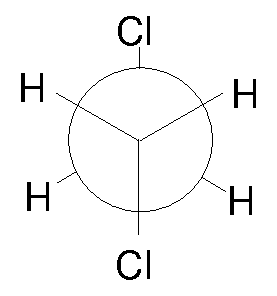
\includegraphics[width=3cm]{1999phy8-4.eps}\\
トランス型
\end{center}
\end{minipage}
\begin{minipage}{.45\linewidth}
\begin{center}
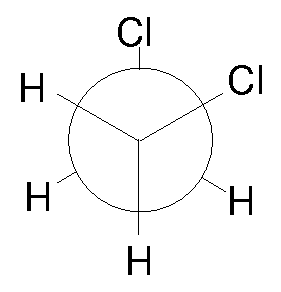
\includegraphics[width=3cm]{1999phy8-5.eps}\\
ゴーシュ型
\end{center}
\end{minipage}\\

\SubSubAnswer この2つの回転異性体におけるC-Cl伸縮運動を考える。

このとき、それぞれの基準振動のモードは以下のようになる。\\

 \begin{minipage}{\linewidth}
 \begin{center}
  \begin{minipage}{.3\linewidth}
   \begin{center}
    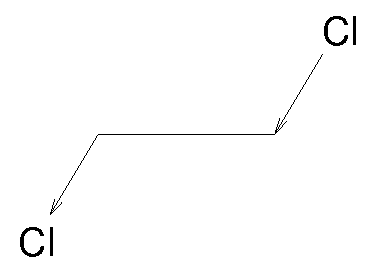
\includegraphics[height=2cm]{1999phy8-6.eps}\\
    トランス型1
   \end{center}
  \end{minipage}
  \hspace{.1\linewidth}
  \begin{minipage}{.3\linewidth}
   \begin{center}
    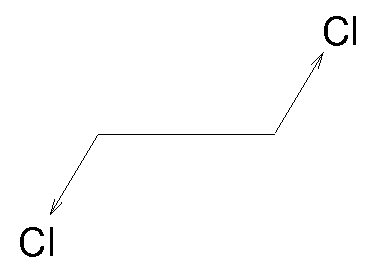
\includegraphics[height=2cm]{1999phy8-7.eps}\\
    トランス型2
   \end{center}
  \end{minipage}
 \end{center}
 \end{minipage}

 \begin{minipage}{\linewidth}
 \begin{center}
  \begin{minipage}{.3\linewidth}
   \begin{center}
    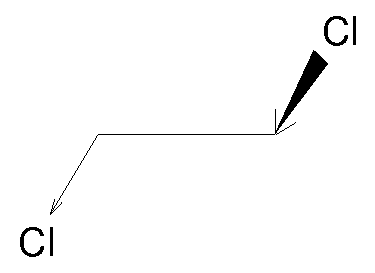
\includegraphics[height=2cm]{1999phy8-8.eps}\\
    ゴーシュ型1
   \end{center}
  \end{minipage}
    \hspace{.1\linewidth}
  \begin{minipage}{.3\linewidth}
   \begin{center}
    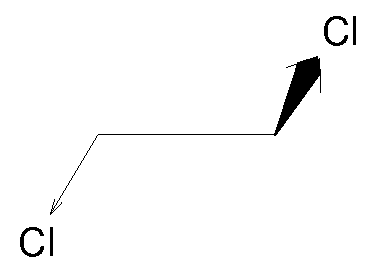
\includegraphics[height=2cm]{1999phy8-9.eps}\\
    ゴーシュ型2
   \end{center}
  \end{minipage}
 \end{center}
 \end{minipage}\\

分子が電磁場と相互作用して光子を吸収あるいは生成するためには分子は少なくとも過渡的に光子に対応する振動数で振動する双極子を持っていなければならない。従って、トランス型2のような双極子モーメントの変化を生じないようなモードはスペクトルに寄与しない。ゆえに、トランス型2を除いたモードが各スペクトルに対応することになる。
\SubSubAnswer バンドの強度比は、それぞれの準位をしめる分子数の比に等しい。この比は、2つの準位間のエネルギー差が$\Delta E$である時、

\begin{minipage}{\linewidth}
\begin{minipage}{.4\linewidth}
\setlength{\unitlength}{1mm}
\begin{picture}(80,35)
\put(10,10){\line(1,0){30}}
\put(10,25){\line(1,0){30}}
\put(12,15){\vector(0,-1){5}}
\put(12,20){\vector(0,1){5}}
\put(5,9){$E_t$}
\put(5,24){$E_g$}
\put(10,16){$\Delta E$}
\put(20,11){占有数$N_t$}
\put(20,26){占有数$N_g$}
\put(45,9){トランス型}
\put(45,5){($g_t$重に縮退)}
\put(45,24){ゴーシュ型}
\put(45,20){($g_g$重に縮退)}
\end{picture}
\end{minipage}
\hspace{.05\linewidth}
\begin{minipage}{.4\linewidth}
\begin{align*}
  \frac{I_{g}(T)}{I_{t}(T)}=\frac{N_{g}(T)}{N_{t}(T)} &= \frac{g_{g}}{g_{t}}\frac{e^{- \beta E_{g}}}{e^{- \beta E_{t}}} \\ &= \frac{g_{g}}{g_{t}} \exp \left[-\frac{\Delta E}{k_{B}T}\right] 
\end{align*}
\end{minipage}
\end{minipage}
と表される。($g_{g}$, $g_{t}$はそれぞれゴーシュ型、トランス型の縮退度である。)

よって、縦軸にこのバンドの強度比の対数を、横軸に$1/T$を取ってグラフ用紙にプロットすると直線になり、その傾きは$- \Delta E/k_{B}$である。これより、$\Delta E$が求まる。
\SubSubAnswer 

ポテンシャルエネルギーの変化は異なった炭素原子に結合している原子同士の回転に伴う電子反発の大きさの変化に由来している。Cl原子はH原子に較べ大きな電子雲を持っているため、Cl-Cl反発やCl-H反発はH-H反発よりも大きなエネルギーを持つ。$\phi = 0,2 \pi$では、Cl-Cl反発が最も大きくなり、また、Cl-H反発も最大になるためポテンシャルエネルギーは最大値を取る。$\phi=2/3 \pi, 4/3 \pi$では、2つのCl-H反発が最大値となるため極大値を取っている。\\
  \begin{center}
    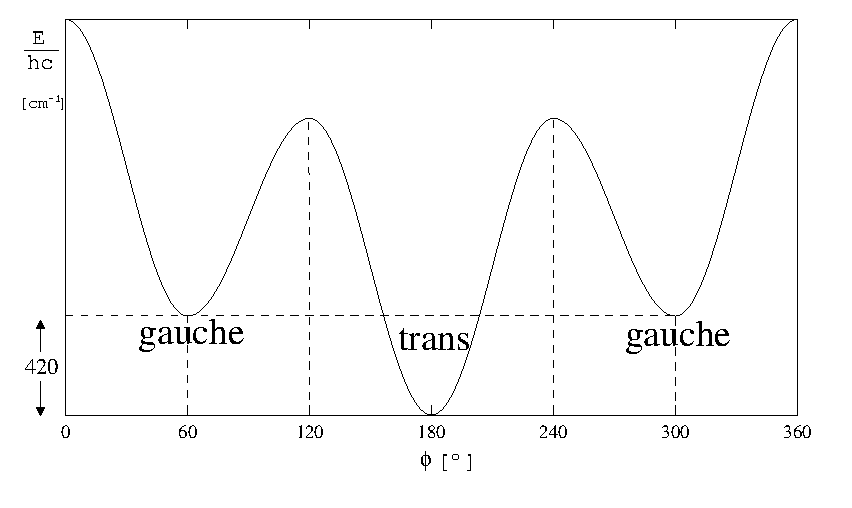
\includegraphics[height=6cm]{1999phy8-10.eps}\\
    ポテンシャルエネルギーの変化
  \end{center}
~\\
 \begin{minipage}{\linewidth}
  \begin{center}
  \begin{minipage}{.2\linewidth}
   \begin{center}
    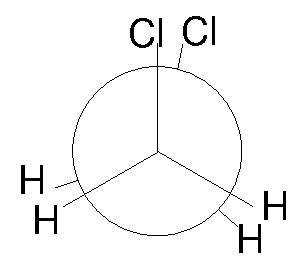
\includegraphics[height=2cm]{1999phy8-11.eps}\\
    $\phi = 0^\circ ,360^\circ$
   \end{center}
  \end{minipage}
  \begin{minipage}{.4\linewidth}
   \begin{center}
    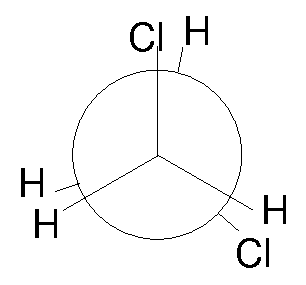
\includegraphics[height=2cm]{1999phy8-12.eps}\\
	$\phi = 120^\circ ,240^\circ$
   \end{center}
  \end{minipage}
  \end{center}
 \end{minipage}\\


\SubSubAnswer
\begin{align*}
\frac{N_{g}}{N_{t}} &= \frac{g_{g}}{g_{t}} \exp \left[-\frac{hc}{k_{B}T}\frac{\Delta E}{hc}\right] \\
                  &= 2 \times 2.7 ^{-\frac{6.6 \times 10^{-34} \times 3 \times 10^{8}}{1.4 \times 10^{-23} \times 290} \times 420 \times 10^{2}}   \\
%                  &\approx 2 \times 2.7^{-2}  \\
                  &= 0.274 \cdots
\end{align*}
ゴーシュ型はトランス型の約27%存在している。
\end{subsubanswers}
\end{subanswers}

\end{answer}


\end{document}
